\documentclass[twoside]{book}

% Packages required by doxygen
\usepackage{fixltx2e}
\usepackage{calc}
\usepackage{doxygen}
\usepackage[export]{adjustbox} % also loads graphicx
\usepackage{graphicx}
\usepackage[utf8]{inputenc}
\usepackage{makeidx}
\usepackage{multicol}
\usepackage{multirow}
\PassOptionsToPackage{warn}{textcomp}
\usepackage{textcomp}
\usepackage[nointegrals]{wasysym}
\usepackage[table]{xcolor}

% Font selection
\usepackage[T1]{fontenc}
\usepackage[scaled=.90]{helvet}
\usepackage{courier}
\usepackage{amssymb}
\usepackage{sectsty}
\renewcommand{\familydefault}{\sfdefault}
\allsectionsfont{%
  \fontseries{bc}\selectfont%
  \color{darkgray}%
}
\renewcommand{\DoxyLabelFont}{%
  \fontseries{bc}\selectfont%
  \color{darkgray}%
}
\newcommand{\+}{\discretionary{\mbox{\scriptsize$\hookleftarrow$}}{}{}}

% Page & text layout
\usepackage{geometry}
\geometry{%
  a4paper,%
  top=2.5cm,%
  bottom=2.5cm,%
  left=2.5cm,%
  right=2.5cm%
}
\tolerance=750
\hfuzz=15pt
\hbadness=750
\setlength{\emergencystretch}{15pt}
\setlength{\parindent}{0cm}
\setlength{\parskip}{3ex plus 2ex minus 2ex}
\makeatletter
\renewcommand{\paragraph}{%
  \@startsection{paragraph}{4}{0ex}{-1.0ex}{1.0ex}{%
    \normalfont\normalsize\bfseries\SS@parafont%
  }%
}
\renewcommand{\subparagraph}{%
  \@startsection{subparagraph}{5}{0ex}{-1.0ex}{1.0ex}{%
    \normalfont\normalsize\bfseries\SS@subparafont%
  }%
}
\makeatother

% Headers & footers
\usepackage{fancyhdr}
\pagestyle{fancyplain}
\fancyhead[LE]{\fancyplain{}{\bfseries\thepage}}
\fancyhead[CE]{\fancyplain{}{}}
\fancyhead[RE]{\fancyplain{}{\bfseries\leftmark}}
\fancyhead[LO]{\fancyplain{}{\bfseries\rightmark}}
\fancyhead[CO]{\fancyplain{}{}}
\fancyhead[RO]{\fancyplain{}{\bfseries\thepage}}
\fancyfoot[LE]{\fancyplain{}{}}
\fancyfoot[CE]{\fancyplain{}{}}
\fancyfoot[RE]{\fancyplain{}{\bfseries\scriptsize Generated by Doxygen }}
\fancyfoot[LO]{\fancyplain{}{\bfseries\scriptsize Generated by Doxygen }}
\fancyfoot[CO]{\fancyplain{}{}}
\fancyfoot[RO]{\fancyplain{}{}}
\renewcommand{\footrulewidth}{0.4pt}
\renewcommand{\chaptermark}[1]{%
  \markboth{#1}{}%
}
\renewcommand{\sectionmark}[1]{%
  \markright{\thesection\ #1}%
}

% Indices & bibliography
\usepackage{natbib}
\usepackage[titles]{tocloft}
\setcounter{tocdepth}{3}
\setcounter{secnumdepth}{5}
\makeindex

% Hyperlinks (required, but should be loaded last)
\usepackage{ifpdf}
\ifpdf
  \usepackage[pdftex,pagebackref=true]{hyperref}
\else
  \usepackage[ps2pdf,pagebackref=true]{hyperref}
\fi
\hypersetup{%
  colorlinks=true,%
  linkcolor=blue,%
  citecolor=blue,%
  unicode%
}

% Custom commands
\newcommand{\clearemptydoublepage}{%
  \newpage{\pagestyle{empty}\cleardoublepage}%
}

\usepackage{caption}
\captionsetup{labelsep=space,justification=centering,font={bf},singlelinecheck=off,skip=4pt,position=top}

%===== C O N T E N T S =====

\begin{document}

% Titlepage & ToC
\hypersetup{pageanchor=false,
             bookmarksnumbered=true,
             pdfencoding=unicode
            }
\pagenumbering{alph}
\begin{titlepage}
\vspace*{7cm}
\begin{center}%
{\Large My Project }\\
\vspace*{1cm}
{\large Generated by Doxygen 1.8.14}\\
\end{center}
\end{titlepage}
\clearemptydoublepage
\pagenumbering{roman}
\tableofcontents
\clearemptydoublepage
\pagenumbering{arabic}
\hypersetup{pageanchor=true}

%--- Begin generated contents ---
\chapter{Namespace Index}
\section{Namespace List}
Here is a list of all documented namespaces with brief descriptions\+:\begin{DoxyCompactList}
\item\contentsline{section}{\mbox{\hyperlink{namespace_p_o__lab1}{P\+O\+\_\+lab1}} }{\pageref{namespace_p_o__lab1}}{}
\end{DoxyCompactList}

\chapter{Hierarchical Index}
\section{Class Hierarchy}
This inheritance list is sorted roughly, but not completely, alphabetically\+:\begin{DoxyCompactList}
\item \contentsline{section}{P\+O\+\_\+lab1.\+Figure\+Choose}{\pageref{class_p_o__lab1_1_1_figure_choose}}{}
\item \contentsline{section}{P\+O\+\_\+lab1.\+Figure\+With\+Single\+Argument}{\pageref{class_p_o__lab1_1_1_figure_with_single_argument}}{}
\begin{DoxyCompactList}
\item \contentsline{section}{P\+O\+\_\+lab1.\+Circle}{\pageref{class_p_o__lab1_1_1_circle}}{}
\item \contentsline{section}{P\+O\+\_\+lab1.\+Square}{\pageref{class_p_o__lab1_1_1_square}}{}
\end{DoxyCompactList}
\item \contentsline{section}{P\+O\+\_\+lab1.\+Figure\+With\+Two\+Arguments}{\pageref{class_p_o__lab1_1_1_figure_with_two_arguments}}{}
\begin{DoxyCompactList}
\item \contentsline{section}{P\+O\+\_\+lab1.\+Rectangle}{\pageref{class_p_o__lab1_1_1_rectangle}}{}
\item \contentsline{section}{P\+O\+\_\+lab1.\+Triangle}{\pageref{class_p_o__lab1_1_1_triangle}}{}
\end{DoxyCompactList}
\item \contentsline{section}{P\+O\+\_\+lab1.\+Program}{\pageref{class_p_o__lab1_1_1_program}}{}
\end{DoxyCompactList}

\chapter{Class Index}
\section{Class List}
Here are the classes, structs, unions and interfaces with brief descriptions\+:\begin{DoxyCompactList}
\item\contentsline{section}{\mbox{\hyperlink{class_p_o__lab1_1_1_circle}{P\+O\+\_\+lab1.\+Circle}} \\*Class lets get a calculated area value. }{\pageref{class_p_o__lab1_1_1_circle}}{}
\item\contentsline{section}{\mbox{\hyperlink{class_p_o__lab1_1_1_figure_choose}{P\+O\+\_\+lab1.\+Figure\+Choose}} \\*Class that calls certain method of calculating area value according to input parameter. }{\pageref{class_p_o__lab1_1_1_figure_choose}}{}
\item\contentsline{section}{\mbox{\hyperlink{class_p_o__lab1_1_1_figure_with_single_argument}{P\+O\+\_\+lab1.\+Figure\+With\+Single\+Argument}} \\*Abstract class that works with figures that need one argument to get area value. }{\pageref{class_p_o__lab1_1_1_figure_with_single_argument}}{}
\item\contentsline{section}{\mbox{\hyperlink{class_p_o__lab1_1_1_figure_with_two_arguments}{P\+O\+\_\+lab1.\+Figure\+With\+Two\+Arguments}} \\*Abstract class that works with figures that need two arguments to get area value. }{\pageref{class_p_o__lab1_1_1_figure_with_two_arguments}}{}
\item\contentsline{section}{\mbox{\hyperlink{class_p_o__lab1_1_1_program}{P\+O\+\_\+lab1.\+Program}} }{\pageref{class_p_o__lab1_1_1_program}}{}
\item\contentsline{section}{\mbox{\hyperlink{class_p_o__lab1_1_1_rectangle}{P\+O\+\_\+lab1.\+Rectangle}} \\*Class lets get a calculated area value. }{\pageref{class_p_o__lab1_1_1_rectangle}}{}
\item\contentsline{section}{\mbox{\hyperlink{class_p_o__lab1_1_1_square}{P\+O\+\_\+lab1.\+Square}} \\*Class lets get a calculated area value. }{\pageref{class_p_o__lab1_1_1_square}}{}
\item\contentsline{section}{\mbox{\hyperlink{class_p_o__lab1_1_1_triangle}{P\+O\+\_\+lab1.\+Triangle}} \\*Class lets get a calculated area value. }{\pageref{class_p_o__lab1_1_1_triangle}}{}
\end{DoxyCompactList}

\chapter{Namespace Documentation}
\hypertarget{namespace_p_o__lab1}{}\section{P\+O\+\_\+lab1 Namespace Reference}
\label{namespace_p_o__lab1}\index{P\+O\+\_\+lab1@{P\+O\+\_\+lab1}}
\subsection*{Classes}
\begin{DoxyCompactItemize}
\item 
class \mbox{\hyperlink{class_p_o__lab1_1_1_circle}{Circle}}
\begin{DoxyCompactList}\small\item\em Class lets get a calculated area value. \end{DoxyCompactList}\item 
class \mbox{\hyperlink{class_p_o__lab1_1_1_figure_choose}{Figure\+Choose}}
\begin{DoxyCompactList}\small\item\em Class that calls certain method of calculating area value according to input parameter. \end{DoxyCompactList}\item 
class \mbox{\hyperlink{class_p_o__lab1_1_1_figure_with_single_argument}{Figure\+With\+Single\+Argument}}
\begin{DoxyCompactList}\small\item\em Abstract class that works with figures that need one argument to get area value. \end{DoxyCompactList}\item 
class \mbox{\hyperlink{class_p_o__lab1_1_1_figure_with_two_arguments}{Figure\+With\+Two\+Arguments}}
\begin{DoxyCompactList}\small\item\em Abstract class that works with figures that need two arguments to get area value. \end{DoxyCompactList}\item 
class \mbox{\hyperlink{class_p_o__lab1_1_1_program}{Program}}
\item 
class \mbox{\hyperlink{class_p_o__lab1_1_1_rectangle}{Rectangle}}
\begin{DoxyCompactList}\small\item\em Class lets get a calculated area value. \end{DoxyCompactList}\item 
class \mbox{\hyperlink{class_p_o__lab1_1_1_square}{Square}}
\begin{DoxyCompactList}\small\item\em Class lets get a calculated area value. \end{DoxyCompactList}\item 
class \mbox{\hyperlink{class_p_o__lab1_1_1_triangle}{Triangle}}
\begin{DoxyCompactList}\small\item\em Class lets get a calculated area value. \end{DoxyCompactList}\end{DoxyCompactItemize}

\chapter{Class Documentation}
\hypertarget{class_p_o__lab1_1_1_circle}{}\section{P\+O\+\_\+lab1.\+Circle Class Reference}
\label{class_p_o__lab1_1_1_circle}\index{P\+O\+\_\+lab1.\+Circle@{P\+O\+\_\+lab1.\+Circle}}


Class lets get a calculated area value.  


Inheritance diagram for P\+O\+\_\+lab1.\+Circle\+:\begin{figure}[H]
\begin{center}
\leavevmode
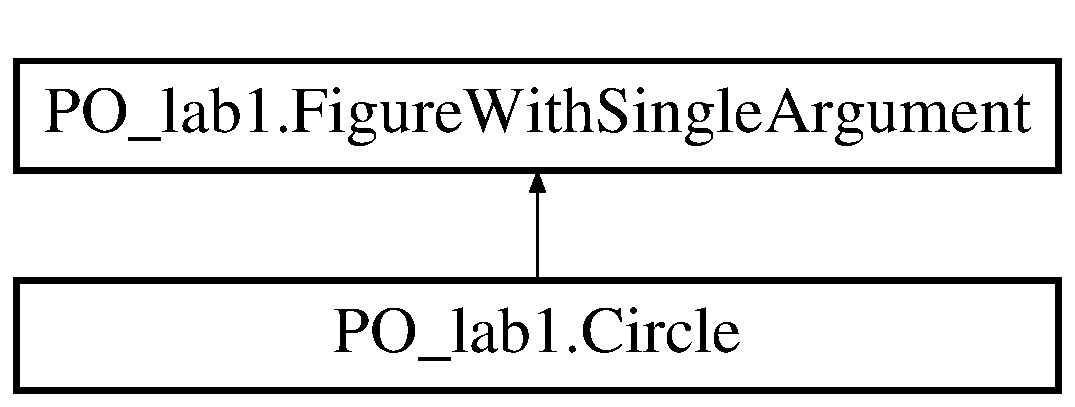
\includegraphics[height=2.000000cm]{class_p_o__lab1_1_1_circle}
\end{center}
\end{figure}
\subsection*{Public Member Functions}
\begin{DoxyCompactItemize}
\item 
override double \mbox{\hyperlink{class_p_o__lab1_1_1_circle_a7eae9033be9ad780426b927e6f841eb8}{Area\+Formula}} (double a)
\begin{DoxyCompactList}\small\item\em Method that calculate area of circle using appropriate formula. \end{DoxyCompactList}\end{DoxyCompactItemize}


\subsection{Detailed Description}
Class lets get a calculated area value. 



\subsection{Member Function Documentation}
\mbox{\Hypertarget{class_p_o__lab1_1_1_circle_a7eae9033be9ad780426b927e6f841eb8}\label{class_p_o__lab1_1_1_circle_a7eae9033be9ad780426b927e6f841eb8}} 
\index{P\+O\+\_\+lab1\+::\+Circle@{P\+O\+\_\+lab1\+::\+Circle}!Area\+Formula@{Area\+Formula}}
\index{Area\+Formula@{Area\+Formula}!P\+O\+\_\+lab1\+::\+Circle@{P\+O\+\_\+lab1\+::\+Circle}}
\subsubsection{\texorpdfstring{Area\+Formula()}{AreaFormula()}}
{\footnotesize\ttfamily override double P\+O\+\_\+lab1.\+Circle.\+Area\+Formula (\begin{DoxyParamCaption}\item[{double}]{a }\end{DoxyParamCaption})\hspace{0.3cm}{\ttfamily [inline]}, {\ttfamily [virtual]}}



Method that calculate area of circle using appropriate formula. 


\begin{DoxyParams}{Parameters}
{\em a} & Arguments needed to calculate area. Radius of circle.\\
\hline
\end{DoxyParams}
\begin{DoxyReturn}{Returns}
Calculated area value.
\end{DoxyReturn}


Implements \mbox{\hyperlink{class_p_o__lab1_1_1_figure_with_single_argument}{P\+O\+\_\+lab1.\+Figure\+With\+Single\+Argument}}.



The documentation for this class was generated from the following file\+:\begin{DoxyCompactItemize}
\item 
Circle.\+cs\end{DoxyCompactItemize}

\hypertarget{class_p_o__lab1_1_1_figure_choose}{}\section{P\+O\+\_\+lab1.\+Figure\+Choose Class Reference}
\label{class_p_o__lab1_1_1_figure_choose}\index{P\+O\+\_\+lab1.\+Figure\+Choose@{P\+O\+\_\+lab1.\+Figure\+Choose}}


Class that calls certain method of calculating area value according to input parameter.  




\subsection{Detailed Description}
Class that calls certain method of calculating area value according to input parameter. 



The documentation for this class was generated from the following file\+:\begin{DoxyCompactItemize}
\item 
Figure\+Choose.\+cs\end{DoxyCompactItemize}

\hypertarget{class_p_o__lab1_1_1_figure_with_single_argument}{}\section{P\+O\+\_\+lab1.\+Figure\+With\+Single\+Argument Class Reference}
\label{class_p_o__lab1_1_1_figure_with_single_argument}\index{P\+O\+\_\+lab1.\+Figure\+With\+Single\+Argument@{P\+O\+\_\+lab1.\+Figure\+With\+Single\+Argument}}


Abstract class that works with figures that need one argument to get area value.  


Inheritance diagram for P\+O\+\_\+lab1.\+Figure\+With\+Single\+Argument\+:\begin{figure}[H]
\begin{center}
\leavevmode
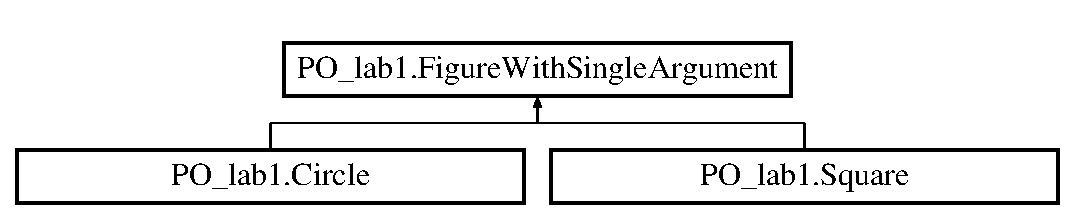
\includegraphics[height=2.000000cm]{class_p_o__lab1_1_1_figure_with_single_argument}
\end{center}
\end{figure}
\subsection*{Public Member Functions}
\begin{DoxyCompactItemize}
\item 
\mbox{\Hypertarget{class_p_o__lab1_1_1_figure_with_single_argument_af248bb28f2247a53ae5979d36ff8ec65}\label{class_p_o__lab1_1_1_figure_with_single_argument_af248bb28f2247a53ae5979d36ff8ec65}} 
abstract double {\bfseries Area\+Formula} (double a)
\item 
double \mbox{\hyperlink{class_p_o__lab1_1_1_figure_with_single_argument_a19718a035b0cc6930df33d05e4e0a92f}{Get\+Area}} (string parameters)
\begin{DoxyCompactList}\small\item\em Method of parsing input parameters and serving it to calculating method. \end{DoxyCompactList}\end{DoxyCompactItemize}


\subsection{Detailed Description}
Abstract class that works with figures that need one argument to get area value. 



\subsection{Member Function Documentation}
\mbox{\Hypertarget{class_p_o__lab1_1_1_figure_with_single_argument_a19718a035b0cc6930df33d05e4e0a92f}\label{class_p_o__lab1_1_1_figure_with_single_argument_a19718a035b0cc6930df33d05e4e0a92f}} 
\index{P\+O\+\_\+lab1\+::\+Figure\+With\+Single\+Argument@{P\+O\+\_\+lab1\+::\+Figure\+With\+Single\+Argument}!Get\+Area@{Get\+Area}}
\index{Get\+Area@{Get\+Area}!P\+O\+\_\+lab1\+::\+Figure\+With\+Single\+Argument@{P\+O\+\_\+lab1\+::\+Figure\+With\+Single\+Argument}}
\subsubsection{\texorpdfstring{Get\+Area()}{GetArea()}}
{\footnotesize\ttfamily double P\+O\+\_\+lab1.\+Figure\+With\+Single\+Argument.\+Get\+Area (\begin{DoxyParamCaption}\item[{string}]{parameters }\end{DoxyParamCaption})\hspace{0.3cm}{\ttfamily [inline]}}



Method of parsing input parameters and serving it to calculating method. 


\begin{DoxyParams}{Parameters}
{\em parameters} & String input parameters.\\
\hline
\end{DoxyParams}
\begin{DoxyReturn}{Returns}
Calculated area value.
\end{DoxyReturn}


The documentation for this class was generated from the following file\+:\begin{DoxyCompactItemize}
\item 
Figure\+With\+Single\+Argument.\+cs\end{DoxyCompactItemize}

\hypertarget{class_p_o__lab1_1_1_figure_with_two_arguments}{}\section{P\+O\+\_\+lab1.\+Figure\+With\+Two\+Arguments Class Reference}
\label{class_p_o__lab1_1_1_figure_with_two_arguments}\index{P\+O\+\_\+lab1.\+Figure\+With\+Two\+Arguments@{P\+O\+\_\+lab1.\+Figure\+With\+Two\+Arguments}}


Abstract class that works with figures that need two arguments to get area value.  


Inheritance diagram for P\+O\+\_\+lab1.\+Figure\+With\+Two\+Arguments\+:\begin{figure}[H]
\begin{center}
\leavevmode
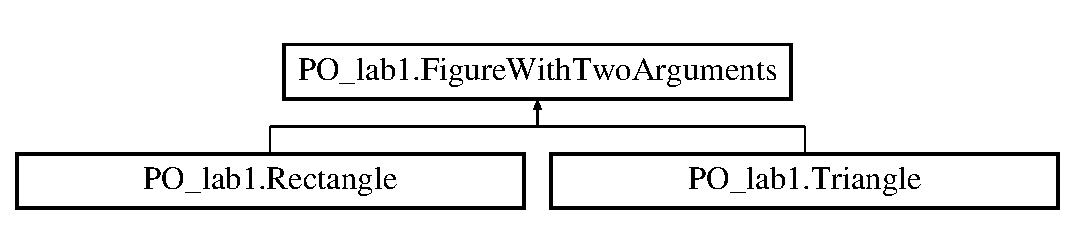
\includegraphics[height=2.000000cm]{class_p_o__lab1_1_1_figure_with_two_arguments}
\end{center}
\end{figure}
\subsection*{Public Member Functions}
\begin{DoxyCompactItemize}
\item 
\mbox{\Hypertarget{class_p_o__lab1_1_1_figure_with_two_arguments_ab3b43a92430a6e866e04ea78627b22eb}\label{class_p_o__lab1_1_1_figure_with_two_arguments_ab3b43a92430a6e866e04ea78627b22eb}} 
abstract double {\bfseries Area\+Formula} (double a, double b)
\item 
double \mbox{\hyperlink{class_p_o__lab1_1_1_figure_with_two_arguments_a443df5d9e9eb30bb0ab7d1af55557af4}{Get\+Area}} (string parameters)
\begin{DoxyCompactList}\small\item\em Method of parsing input parameters and serving it to calculating method. \end{DoxyCompactList}\end{DoxyCompactItemize}


\subsection{Detailed Description}
Abstract class that works with figures that need two arguments to get area value. 



\subsection{Member Function Documentation}
\mbox{\Hypertarget{class_p_o__lab1_1_1_figure_with_two_arguments_a443df5d9e9eb30bb0ab7d1af55557af4}\label{class_p_o__lab1_1_1_figure_with_two_arguments_a443df5d9e9eb30bb0ab7d1af55557af4}} 
\index{P\+O\+\_\+lab1\+::\+Figure\+With\+Two\+Arguments@{P\+O\+\_\+lab1\+::\+Figure\+With\+Two\+Arguments}!Get\+Area@{Get\+Area}}
\index{Get\+Area@{Get\+Area}!P\+O\+\_\+lab1\+::\+Figure\+With\+Two\+Arguments@{P\+O\+\_\+lab1\+::\+Figure\+With\+Two\+Arguments}}
\subsubsection{\texorpdfstring{Get\+Area()}{GetArea()}}
{\footnotesize\ttfamily double P\+O\+\_\+lab1.\+Figure\+With\+Two\+Arguments.\+Get\+Area (\begin{DoxyParamCaption}\item[{string}]{parameters }\end{DoxyParamCaption})\hspace{0.3cm}{\ttfamily [inline]}}



Method of parsing input parameters and serving it to calculating method. 


\begin{DoxyParams}{Parameters}
{\em parameters} & String input parameters.\\
\hline
\end{DoxyParams}
\begin{DoxyReturn}{Returns}
Calculated area value.
\end{DoxyReturn}


The documentation for this class was generated from the following file\+:\begin{DoxyCompactItemize}
\item 
Figure\+With\+Two\+Arguments.\+cs\end{DoxyCompactItemize}

\hypertarget{class_p_o__lab1_1_1_program}{}\section{P\+O\+\_\+lab1.\+Program Class Reference}
\label{class_p_o__lab1_1_1_program}\index{P\+O\+\_\+lab1.\+Program@{P\+O\+\_\+lab1.\+Program}}


The documentation for this class was generated from the following file\+:\begin{DoxyCompactItemize}
\item 
Program.\+cs\end{DoxyCompactItemize}

\hypertarget{class_p_o__lab1_1_1_rectangle}{}\section{P\+O\+\_\+lab1.\+Rectangle Class Reference}
\label{class_p_o__lab1_1_1_rectangle}\index{P\+O\+\_\+lab1.\+Rectangle@{P\+O\+\_\+lab1.\+Rectangle}}


Class lets get a calculated area value.  


Inheritance diagram for P\+O\+\_\+lab1.\+Rectangle\+:\begin{figure}[H]
\begin{center}
\leavevmode
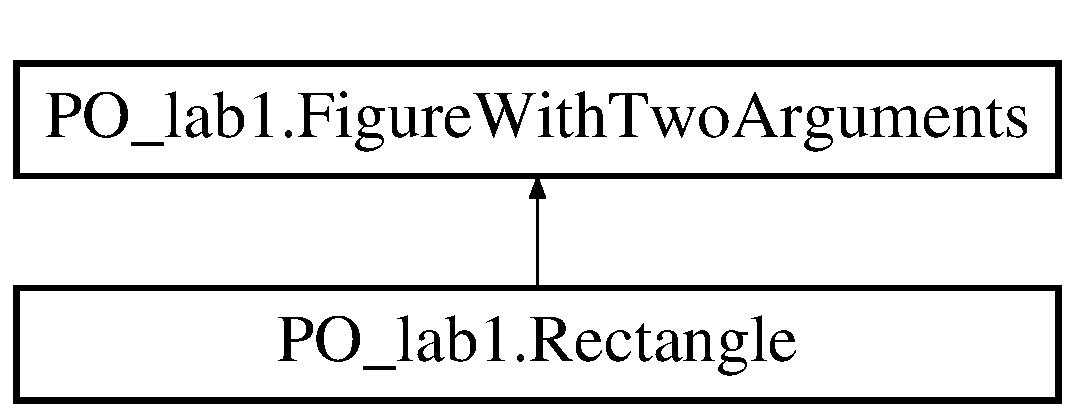
\includegraphics[height=2.000000cm]{class_p_o__lab1_1_1_rectangle}
\end{center}
\end{figure}
\subsection*{Public Member Functions}
\begin{DoxyCompactItemize}
\item 
override double \mbox{\hyperlink{class_p_o__lab1_1_1_rectangle_a14f4a197dc43f0b6ea2063f87a89e451}{Area\+Formula}} (double a, double b)
\begin{DoxyCompactList}\small\item\em Method that calculate area of rectangle using appropriate formula. \end{DoxyCompactList}\end{DoxyCompactItemize}


\subsection{Detailed Description}
Class lets get a calculated area value. 



\subsection{Member Function Documentation}
\mbox{\Hypertarget{class_p_o__lab1_1_1_rectangle_a14f4a197dc43f0b6ea2063f87a89e451}\label{class_p_o__lab1_1_1_rectangle_a14f4a197dc43f0b6ea2063f87a89e451}} 
\index{P\+O\+\_\+lab1\+::\+Rectangle@{P\+O\+\_\+lab1\+::\+Rectangle}!Area\+Formula@{Area\+Formula}}
\index{Area\+Formula@{Area\+Formula}!P\+O\+\_\+lab1\+::\+Rectangle@{P\+O\+\_\+lab1\+::\+Rectangle}}
\subsubsection{\texorpdfstring{Area\+Formula()}{AreaFormula()}}
{\footnotesize\ttfamily override double P\+O\+\_\+lab1.\+Rectangle.\+Area\+Formula (\begin{DoxyParamCaption}\item[{double}]{a,  }\item[{double}]{b }\end{DoxyParamCaption})\hspace{0.3cm}{\ttfamily [inline]}, {\ttfamily [virtual]}}



Method that calculate area of rectangle using appropriate formula. 


\begin{DoxyParams}{Parameters}
{\em a} & Argument needed to calculate area.\\
\hline
{\em b} & Argument needed to calculate area.\\
\hline
\end{DoxyParams}
\begin{DoxyReturn}{Returns}
Calculated area value.
\end{DoxyReturn}


Implements \mbox{\hyperlink{class_p_o__lab1_1_1_figure_with_two_arguments}{P\+O\+\_\+lab1.\+Figure\+With\+Two\+Arguments}}.



The documentation for this class was generated from the following file\+:\begin{DoxyCompactItemize}
\item 
Rectangle.\+cs\end{DoxyCompactItemize}

\hypertarget{class_p_o__lab1_1_1_square}{}\section{P\+O\+\_\+lab1.\+Square Class Reference}
\label{class_p_o__lab1_1_1_square}\index{P\+O\+\_\+lab1.\+Square@{P\+O\+\_\+lab1.\+Square}}


Class lets get a calculated area value.  


Inheritance diagram for P\+O\+\_\+lab1.\+Square\+:\begin{figure}[H]
\begin{center}
\leavevmode
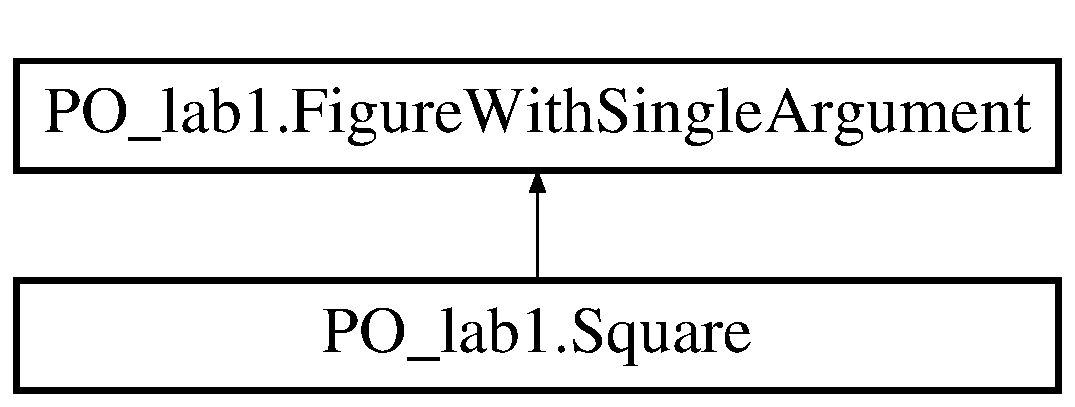
\includegraphics[height=2.000000cm]{class_p_o__lab1_1_1_square}
\end{center}
\end{figure}
\subsection*{Public Member Functions}
\begin{DoxyCompactItemize}
\item 
override double \mbox{\hyperlink{class_p_o__lab1_1_1_square_aac1ad97365aabd8b19ae4058b834dd8d}{Area\+Formula}} (double a)
\begin{DoxyCompactList}\small\item\em Method that calculate area of square using appropriate formula. \end{DoxyCompactList}\end{DoxyCompactItemize}


\subsection{Detailed Description}
Class lets get a calculated area value. 



\subsection{Member Function Documentation}
\mbox{\Hypertarget{class_p_o__lab1_1_1_square_aac1ad97365aabd8b19ae4058b834dd8d}\label{class_p_o__lab1_1_1_square_aac1ad97365aabd8b19ae4058b834dd8d}} 
\index{P\+O\+\_\+lab1\+::\+Square@{P\+O\+\_\+lab1\+::\+Square}!Area\+Formula@{Area\+Formula}}
\index{Area\+Formula@{Area\+Formula}!P\+O\+\_\+lab1\+::\+Square@{P\+O\+\_\+lab1\+::\+Square}}
\subsubsection{\texorpdfstring{Area\+Formula()}{AreaFormula()}}
{\footnotesize\ttfamily override double P\+O\+\_\+lab1.\+Square.\+Area\+Formula (\begin{DoxyParamCaption}\item[{double}]{a }\end{DoxyParamCaption})\hspace{0.3cm}{\ttfamily [inline]}, {\ttfamily [virtual]}}



Method that calculate area of square using appropriate formula. 


\begin{DoxyParams}{Parameters}
{\em a} & Arguments needed to calculate area. Side of square.\\
\hline
\end{DoxyParams}
\begin{DoxyReturn}{Returns}
Calculated area value.
\end{DoxyReturn}


Implements \mbox{\hyperlink{class_p_o__lab1_1_1_figure_with_single_argument}{P\+O\+\_\+lab1.\+Figure\+With\+Single\+Argument}}.



The documentation for this class was generated from the following file\+:\begin{DoxyCompactItemize}
\item 
Square.\+cs\end{DoxyCompactItemize}

\hypertarget{class_p_o__lab1_1_1_triangle}{}\section{P\+O\+\_\+lab1.\+Triangle Class Reference}
\label{class_p_o__lab1_1_1_triangle}\index{P\+O\+\_\+lab1.\+Triangle@{P\+O\+\_\+lab1.\+Triangle}}


Class lets get a calculated area value.  


Inheritance diagram for P\+O\+\_\+lab1.\+Triangle\+:\begin{figure}[H]
\begin{center}
\leavevmode
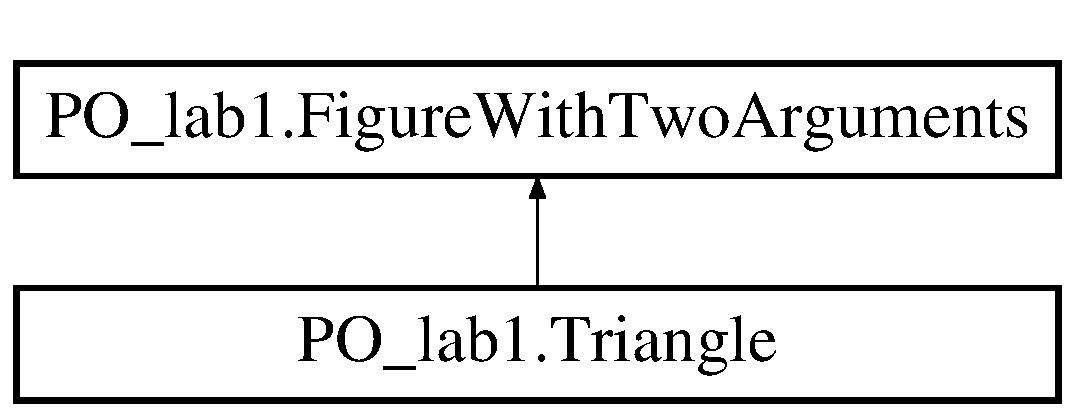
\includegraphics[height=2.000000cm]{class_p_o__lab1_1_1_triangle}
\end{center}
\end{figure}
\subsection*{Public Member Functions}
\begin{DoxyCompactItemize}
\item 
override double \mbox{\hyperlink{class_p_o__lab1_1_1_triangle_aa4e000e20ad3f9b88b90b435c8b4d3ec}{Area\+Formula}} (double a, double b)
\begin{DoxyCompactList}\small\item\em Method that calculate area of triangle using appropriate formula. \end{DoxyCompactList}\end{DoxyCompactItemize}


\subsection{Detailed Description}
Class lets get a calculated area value. 



\subsection{Member Function Documentation}
\mbox{\Hypertarget{class_p_o__lab1_1_1_triangle_aa4e000e20ad3f9b88b90b435c8b4d3ec}\label{class_p_o__lab1_1_1_triangle_aa4e000e20ad3f9b88b90b435c8b4d3ec}} 
\index{P\+O\+\_\+lab1\+::\+Triangle@{P\+O\+\_\+lab1\+::\+Triangle}!Area\+Formula@{Area\+Formula}}
\index{Area\+Formula@{Area\+Formula}!P\+O\+\_\+lab1\+::\+Triangle@{P\+O\+\_\+lab1\+::\+Triangle}}
\subsubsection{\texorpdfstring{Area\+Formula()}{AreaFormula()}}
{\footnotesize\ttfamily override double P\+O\+\_\+lab1.\+Triangle.\+Area\+Formula (\begin{DoxyParamCaption}\item[{double}]{a,  }\item[{double}]{b }\end{DoxyParamCaption})\hspace{0.3cm}{\ttfamily [inline]}, {\ttfamily [virtual]}}



Method that calculate area of triangle using appropriate formula. 


\begin{DoxyParams}{Parameters}
{\em a} & Argument needed to calculate area.\\
\hline
{\em b} & Argument needed to calculate area.\\
\hline
\end{DoxyParams}
\begin{DoxyReturn}{Returns}
Calculated area value.
\end{DoxyReturn}


Implements \mbox{\hyperlink{class_p_o__lab1_1_1_figure_with_two_arguments}{P\+O\+\_\+lab1.\+Figure\+With\+Two\+Arguments}}.



The documentation for this class was generated from the following file\+:\begin{DoxyCompactItemize}
\item 
Triangle.\+cs\end{DoxyCompactItemize}

%--- End generated contents ---

% Index
\backmatter
\newpage
\phantomsection
\clearemptydoublepage
\addcontentsline{toc}{chapter}{Index}
\printindex

\end{document}
